\documentclass[12pt]{article}
\usepackage{float}
\usepackage{caption, subcaption}
\usepackage[T1]{fontenc}
\usepackage[backend=bibtex, maxbibnames=99, sorting=none]{biblatex}
\addbibresource{sample.bib}
\usepackage{url}
\usepackage[utf8]{inputenc}
\usepackage{amsmath}
\usepackage{setspace}
\usepackage{graphicx}
\graphicspath{{Images/}}
\usepackage{parskip}
\usepackage{multirow}
\usepackage{enumitem}
\usepackage{amssymb}
\usepackage{framed}
\usepackage{fancyhdr}
\usepackage{vmargin}
\usepackage{subcaption} %usamos subcaption mejor que subfig (más moderno)
\usepackage{eurosym}
\usepackage[table,xcdraw]{xcolor} % add color to your tables
\usepackage[bottom]{footmisc} %footnotes
\definecolor{blau}{RGB}{210,235,255}
\definecolor{blau2}{RGB}{120,170,225}
\setmarginsrb{2.5 cm}{2 cm}{2 cm}{2.5 cm}{1 cm}{0.5 cm}{1 cm}{1 cm}

\usepackage{multirow}

\usepackage{chngcntr}

\usepackage[framed, numbered]{matlab-prettifier}
 
\counterwithin{figure}{section}
\counterwithin{table}{section}
\numberwithin{equation}{section}

\usepackage{titlesec}
\usepackage{hyperref}
\usepackage{listings}
\usepackage{multicol}
\setlength{\columnsep}{1cm}

\titleclass{\subsubsubsection}{straight}[\subsection]

\newcounter{subsubsubsection}[subsubsection]
\renewcommand\thesubsubsubsection{\thesubsubsection.\arabic{subsubsubsection}}
\renewcommand\theparagraph{\thesubsubsubsection.\arabic{paragraph}} % optional; useful if paragraphs are to be numbered

\titleformat{\subsubsubsection}
  {\normalfont\normalsize\bfseries}{\thesubsubsubsection}{1em}{}
\titlespacing*{\subsubsubsection}
{0pt}{3.25ex plus 1ex minus .2ex}{1.5ex plus .2ex}

\makeatletter
\renewcommand\paragraph{\@startsection{paragraph}{5}{\z@}%
  {3.25ex \@plus1ex \@minus.2ex}%
  {-1em}%
  {\normalfont\normalsize\bfseries}}
\renewcommand\subparagraph{\@startsection{subparagraph}{6}{\parindent}%
  {3.25ex \@plus1ex \@minus .2ex}%
  {-1em}%
  {\normalfont\normalsize\bfseries}}
\def\toclevel@subsubsubsection{4}
\def\toclevel@paragraph{5}
\def\toclevel@paragraph{6}
\def\l@subsubsubsection{\@dottedtocline{4}{7em}{4em}}
\def\l@paragraph{\@dottedtocline{5}{10em}{5em}}
\def\l@subparagraph{\@dottedtocline{6}{14em}{6em}}
\makeatother

\usepackage[table,xcdraw]{xcolor}

\setcounter{secnumdepth}{4}
\setcounter{tocdepth}{4}


\usepackage{pdflscape} %Per poder posar la pàgina en horizontal
\usepackage{multicol} %Escriure en columnes 
 
	% Author
\date{\today}							% Date

\makeatletter
\let\thetitle\@title
\let\theauthor\@author
\let\thedate\@date
\makeatother

\pagestyle{fancy}
\fancyhf{}
\lhead{21D009 Networks: Concepts and Algorithms}
\rhead{Movie recommendations using networks}
\cfoot{\thepage}

\begin{document}

\begin{titlepage}
	\centering
    
\includegraphics[scale = 0.7]{bse_logo.png}\\[1.2 cm]	% University Logo
    \textsc{\LARGE Barcelona School of Economics}\\[2.0 cm]	% University Name
	\textsc{\Large Data Science Methodology Program}\\[0.5 cm]				% Course Code
	\textsc{\large 21D009 Networks: Concepts and Algorithms }\\[0.5 cm]				% Course Name
	\rule{\linewidth}{0.2 mm} \\[0.4 cm]
	{ \huge \bfseries Movie recommendations using networks }\\
	\rule{ \linewidth}{0.2 mm} \\[1.5 cm]
	
\begin{center}
    
{ \emph{Authors: }\\
    \textsc{Codd}, Jonny \\
    \textsc{Chen}, Joshua \\
    \textsc{Gallegos}, Rafael \\
    \textsc{Pérez}, Carlos \\ } 

\vspace{0.7cm}


    \textit{Professors:}\\  \textsc{Milán}, Pau \\
    	\textsc{Komander}, Björn
        \\ \vspace{0.5cm}


\vspace{1.7cm}


{\large December $20^{th}$, 2023} \\[2 cm]

 \end{center}
	\vfill
	
\end{titlepage}
	
\tableofcontents
\vspace{1cm}
\listoffigures
\listoftables
\pagebreak

\newpage

\section{Introduction}

The travelling salesman problem (TSP) is an archetypal problem in linear programming. The setup tells the reader to imagine a salesman who must visit \textit{n} cities, then asks them to find the shortest path the salesman can take, visiting each city exactly once before returning to the starting city given the distance between all pairs of cities. Its deceptively simple formulation lies in stark contrast to the vast computational expense required to solve it; it is NP-hard, and despite nearly one-hundred years of literature, we rely on heuristic algorithms to find good solutions. 

\section{Dataset}

MovieLens is a recommender system that was developed by GroupLens, a computer science research lab at the University of Minnesota. The goal of this challenge is to recommend movies to its users based on their movie ratings. Group Lens offers datasets of different sizes and their datasets are widely used in research and teaching contexts.

The selected dataset consists mainly on two files: movies.csv and ratings.csv. Movies dataset has 9742 unique films and a column indicating the genres of the film. All possible genres are: 'Romance', 'Musical', 'Children', 'Documentary', 'Sci-Fi', 'Film-Noir', '(no genres listed)', 'Crime', 'Mystery', 'Drama', 'Western', 'Fantasy', 'Animation', 'Thriller', 'War', 'Action', 'Adventure', 'IMAX', 'Comedy', 'Horror'. The number of movies per genre is represented in Figure \ref{fig:count_genre}.

Ratings dataset consists of 100836 ratings with 610 unique users that rated 9724 movies. As it can be observed in Figure \ref{fig:count_ratings}, the ratings from users are high, which suggests that users tend to enter or register their rating on movies that they probably have liked. 

\begin{figure}[h!]
 \end{figure}

\begin{figure}[h!]
    \begin{minipage}[b]{0.49\linewidth}
         \centering
  	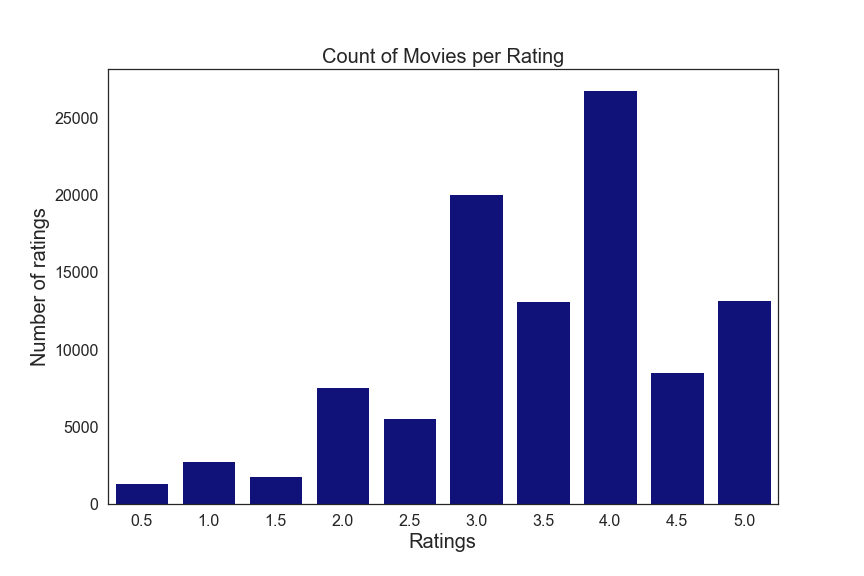
\includegraphics[width=0.99\textwidth]{count_rating.png}
  	\caption{Count of Movies per Rating}
  	\label{fig:count_ranking}
    \end{minipage}
    \hspace{0.01cm}
    \begin{minipage}[b]{0.49\linewidth}
        \centering
  	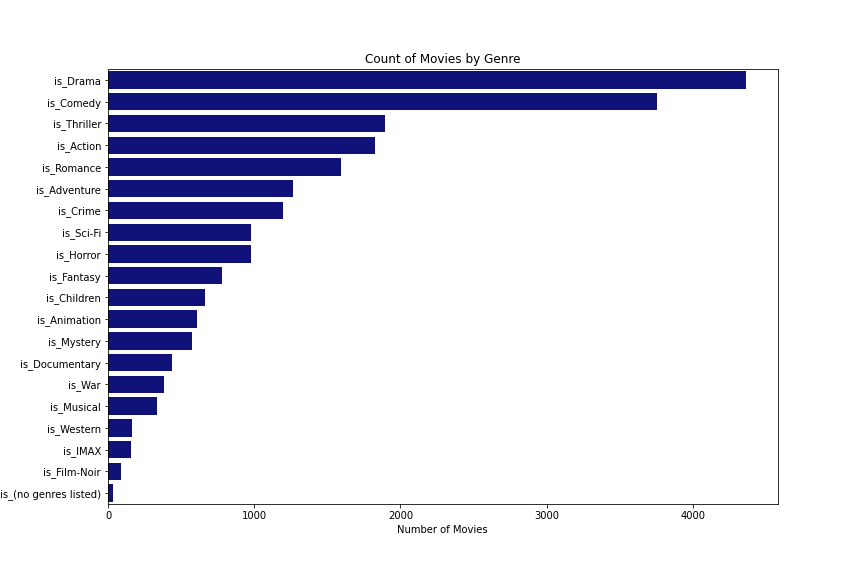
\includegraphics[width=0.99\textwidth]{count_genre.png}
  	\caption{Count of Movies per Genre}
  	\label{fig:count_genre}
    \end{minipage}
\end{figure}

\section{Network analysis}

\subsection{User-to-user network}

\subsection{Movie-to-Movie network}

\subsection{User and movie bipartite network}

\begin{subequations}
\renewcommand{\theequation}{1.\arabic{equation}}

\begin{align}
\min \quad & \sum_{i \in V} \sum_{j \in V\setminus\{i\}} c_{ij}x_{ij} \\
\text{s.t.} \quad & \sum_{j \in V\setminus\{i\}} x_{ij} = 1 & \forall i \in V \\
& \sum_{j \in V\setminus\{i\}} x_{ji} = 1 & \forall i \in V \\
& \sum_{i \in S} \sum_{j \in V\setminus S} x_{ij} \geq 1 & \forall S \subseteq V, S \neq \emptyset \\
& x_{ij} \in \{0,1\} & \forall i \in V, \forall j \in V \setminus \{i\}.
\end{align}

\text{where:}
\begin{itemize}
    \item \( V \) is the set of cities.
    \item \( c_{ij} \) is the cost or distance from city \( i \) to city \( j \).
    \item \( x_{ij} \) is a binary variable that equals 1 if the path from city \( i \) to city \( j \) is included in the tour, and 0 otherwise.
    \item \( S \) is any subset of cities. The subtour elimination constraints (SECs) ensure that for any subset of cities \( S \), there is at least one path leading out of the subset to prevent the formation of subtours. This is crucial for ensuring that the solution is a single tour covering all cities, rather than multiple disconnected tours.
\end{itemize}

\end{subequations}


\vspace{1em}

\textit{\small The ATSP asks the program to find the minimum distance the salesman must travel according to the following constraints: each city must be entered exactly once; each city must be left exactly once; subtours are not allowed.}

All implementations have been developed in Python. The source code can be found in the attached jupyter notebook \textit{TSP$\_$project.ipynb}.

\vspace{1em} 

\subsection{Algorithms}

\textbf{Integer Branch-and-Price:} For a sufficiently large \textit{n} (which, in practice, is relatively small), specifying the exclusion of all SECs is computationally infeasible. As \textit{n} increases, the number of SECs increases exponentially with $2^n$ (\textit{n} representing the number of cities).

The Integer Branch-and-Price algorithm circumnavigates the computational burden by first solving a relaxed form of the problem which initially ignores the exclusion of subtours. Once the algorithm finds a feasible integer solution to the relaxed problem, it checks for subtours and adds SECs to the original formulation. 

\begin{equation}
\sum_{i \in S_l} \sum_{j \in V \backslash S_l} x_{ij} \geq 1 \quad \quad \forall l \in \{1, ...., k \}
\end{equation}

with \textit{k} representing the number of SECs violated while searching for the optimal solution.\\

\noindent\textbf{Fractional Branch-and-Price:} The fractional Branch-and-Price algorithm is less stringent in restricting solutions to the relaxed problem. Instead of waiting until the algorithm produces a feasible integer solution, it accepts fractional solutions and checks for violated SECs using the Max Flow Problem. If an SEC is violated, it is added as a constraint.

\begin{equation}
\sum_{i \in S} \sum_{j \in V \backslash S} x_{ij} \ge 1 \quad \quad \exists S  \subseteq V , S  \ne \emptyset 
\end{equation}

The Boykov Kolmogorov Max Flow algorithm from graph$\_$tool python package is used to solve the Max Flow problem. Max Flow detects violated SECs from any vertex to all other vertices in the subtour; if the obtained max flow is less than 1, we add the violated SEC as a constraint.

Once an integer solution with no subtours is found, both algorithms branch the search at variables of interest to look for better solutions. The algorithms are terminated either when an exhaustive search has been performed, or a specified time limit on computation has been reached.\\

We subset the data to produce instances of varying size and calculate the time taken to reach the optimal solution (if it is indeed reached); the number of iterations; and the final objective value. The algorithms are limited to a maximum run time of five minutes. If they fail to terminate within this limit, we report a solve time of 300 seconds.

When run on ATSP datasets, both solvers reached the optimal solution in reasonable time. However, in symmetric cases with a comparable number of nodes, the solver took much longer. We found the problems in \cite{web:tsp} to be more challenging to solve, even though they are symmetric. This finding was surprising, as we expected the algorithm to leverage the symmetries in the distance matrices to reduce computation time. We believe the longer running times should be attributed to more challenging initial parameters in these datasets, rather than to the symmetric property. 

\section{Task 1}

 We found that the integer algorithm was far more efficient across all subsets of our problem. It consistently took less time to converge than the fractional algorithm (Figure 2.1), and the difference in time generally grew as the number of vertices increased. This suggests permitting further relaxation of the constraints of the initial problem (i.e., allowing non-integer solutions), then readmitting them later where necessary, is less efficient, at least in terms of computation time, than simply including the constraints from the beginning. 
 
 Aditionally, the runtime limit was reached in the instance of the fractional solver with 350 vertices, so no useful statistics were output. Interestingly, though, in the case with 400 vertices the problem was solved by the fractional algorithm before the limit was reached, suggesting that adding the additional data points made the problem easier to solve. From this finding we inferred that, while the integer algorithm finds a solution more quickly than the fractional algorithm, the exact time difference depends on the parameters of the problem. In cases in which both algorithms converged within the time limit, their objective values were consistent. Overall this analysis implies that both algorithms are accurate, but the integer variant is quicker. 
 
 Finally, we discerned no clear pattern between the number of iterations in the integer vs fractional solver.

\vspace{1em}
\begin{table}[!ht]
\centering
\begin{tabular}{|c|c|c|c|c|c|c|c|}
\hline
\textbf{Vertices} & \multicolumn{3}{c|}{\textbf{Integer}} & \multicolumn{3}{c|}{\textbf{Fractional}} \\
\hline
 & \textbf{Obj} & \textbf{Iter} & \textbf{Time} & \textbf{Obj} & \textbf{Iter} & \textbf{Time} \\
\hline
      43 &           398 &            365 &           0.15 &              398 &               179 &              0.76 \\
      93 &           564 &            475 &           0.27 &              564 &             1,017 &              4.20 \\
     143 &           907 &          3,720 &           4.20 &              907 &             3,120 &              8.52 \\
     193 &          1196 &          8,973 &           4.05 &             1196 &             7,771 &             82.40 \\
     243 &          1645 &         13,792 &           9.57 &             1645 &             9,642 &             49.11 \\
     293 &          1807 &         12,784 &          16.24 &             1807 &            14,346 &             78.40 \\
     343 &          2071 &         20,397 &          19.71 &                NA &                 NA &            300.00 \\
     393 &          2383 &         45,017 &          59.09 &             2383 &            41,738 &             75.83 \\
     443 &          2720 &         25,485 &          53.19 &             2720 &            42,299 &             89.35 \\
\hline
\end{tabular}
\caption{Objective Value, Iterations, and Runtime for Integer and Fractional algorithms}
\label{table:separated_comparison}
\end{table}

\vspace{1em} 

\newpage
\section{Task 2}

It is computationally impractical to add all SECs to the original LP, so we adopt a more parsimonious approach in an effort to enhance solving efficiency and reduce overall computation time. In particular, we first remove all sub tours of length two and, subsequently, those of length three.\\

\vspace{1em}


\begin{table}[!ht]
\centering
\begin{tabular}{|c|c|c|c|c|c|c|c|c|c|}
\hline
\textbf{Vertices} & \multicolumn{3}{c|}{\textbf{No constraints}} & \multicolumn{3}{c|}{\textbf{Cardinality 2}} & \multicolumn{3}{c|}{\textbf{Cardinality 3}} \\
\hline
 & \textbf{Obj} & \textbf{Iter} & \textbf{Time} & \textbf{Obj} & \textbf{Iter} & \textbf{Time} & \textbf{Obj} & \textbf{Iter} & \textbf{Time} \\
\hline
     43 &                  398 &                   365 &                  0.15 &                 398 &                  193 &                 0.38 &                 398 &                  348 &                 0.21 \\
      93 &                  564 &                   475 &                  0.27 &                 564 &                  390 &                 0.53 &                 564 &                  520 &                 1.51 \\
     143 &                  907 &                 3,720 &                  4.20 &                 907 &                2,029 &                 1.78 &                 907 &                  918 &                10.81 \\
     193 &                1,196 &                 8,973 &                  4.05 &               1,196 &                2,666 &                 7.87 &               1,196 &                2,854 &                39.35 \\
     243 &                1,645 &                13,792 &                  9.57 &               1,645 &                4,552 &                 7.75 &               1,645 &                4,222 &               136.02 \\
     293 &                1,807 &                12,784 &                 16.24 &               1,807 &                6,134 &                17.13 &                   NA &                    NA &               300.00 \\
     343 &                2,071 &                20,397 &                 19.71 &               2,071 &                1,856 &                10.32 &                   NA &                    NA &               300.00 \\
     393 &                2,383 &                45,017 &                 59.09 &               2,383 &                9,184 &                30.64 &                   NA &                    NA &               300.00 \\
     443 &                2,720 &                25,485 &                 53.19 &               2,720 &                5,779 &                30.29 &                   NA &                    NA &               300.00 \\
\hline
\end{tabular}
\caption{Objective Value, Iterations, and Runtime for the Integer algorithm with SECs of cardinality 2 and 3}
\label{table:q2 - int}
\end{table}

\vspace{1em} 

\noindent\textbf{Fractional Branch-and-Price:} By making the initial relaxation tighter, we attenuate the numerical distance between the relaxed solution and the optimal integer solution. This reduces the number of nodes in the branch-and-bound tree, as fewer branches are needed to transform the fractional solution of the relaxation into the integer solution. Conversely, adding many SECs upfront increases the size and complexity of the constraint matrix the solver is confronted with at each node in the branch-and-bound tree. This extra computational expense likely increases solving time. \\

\noindent Table \ref{table:q2 - frac} summarizes the results for the fractional solver. As for the integer solver, adding SECs of cardinality 2 and 3 reduced the number of iterations required to find the optimal solution (if it was indeed reached). However, SECs of cardinality 2 improved the performance of the algorithm, with reduced computation time (Figure 3.1) and the optimal solution was found in time in all instances. This implies the reduction in required iterations offset the increased computational cost of checking additional constraints. Conversely, SECs of cardinality 3 generally hindered performance, with no optimal solution found in instances of over 293 vertices.


\begin{table}[!ht]
\centering
\begin{tabular}{|c|c|c|c|c|c|c|c|c|c|}
\hline
\textbf{Vertices} & \multicolumn{3}{c|}{\textbf{No constraints}} & \multicolumn{3}{c|}{\textbf{Cardinality 2}} & \multicolumn{3}{c|}{\textbf{Cardinality 3}} \\
\hline
 & \textbf{Obj} & \textbf{Iter} & \textbf{Time} & \textbf{Obj} & \textbf{Iter} & \textbf{Time} & \textbf{Obj} & \textbf{Iter} & \textbf{Time} \\
\hline
      43 &                  398 &                   179 &                  0.76 &                 398 &                  171 &                 0.36 &                 398 &                  189 &                 1.04 \\
      93 &                  564 &                 1,017 &                  4.20 &                 564 &                  401 &                 3.90 &                 564 &                  520 &                 2.60 \\
     143 &                  907 &                 3,120 &                  8.52 &                 907 &                1,662 &                18.38 &                 907 &                1,824 &                28.63 \\
     193 &                1,196 &                 7,771 &                 82.40 &               1,196 &                3,727 &                17.15 &               1,196 &                2,685 &                47.84 \\
     243 &                1,645 &                 9,642 &                 49.11 &               1,645 &                5,191 &                28.35 &               1,645 &                3,713 &               109.35 \\
     293 &                1,807 &                14,346 &                 78.40 &               1,807 &                4,510 &                27.43 &                 NaN &                  NaN &               300.00 \\
     343 &                  NaN &                   NaN &                300.00 &               2,071 &                8,283 &               103.88 &                 NaN &                  NaN &               300.00 \\
     393 &                2,383 &                41,738 &                 75.83 &               2,383 &                9,924 &               271.21 &                 NaN &                  NaN &               300.00 \\
     443 &                2,720 &                42,299 &                 89.35 &               2,720 &               12,923 &               240.33 &                 NaN &                  NaN &               300.00 \\
\hline
\end{tabular}
\caption{Objective Value, Iterations, and Runtime for the Integer algorithm with SECs of cardinality 2 and 3}
\label{table:q2 - frac}
\end{table}

\newpage
\section{Task 3}
\vspace{1em} 


\begin{table}[ht]
\centering
\begin{tabular}{c|ccc|ccc|}
\cline{2-7}
\multicolumn{1}{l|}{}                 & \multicolumn{3}{c|}{\textbf{\begin{tabular}[c]{@{}c@{}}Integer\\ (2720 - 25,485 iter - 53.19s)\end{tabular}}} & \multicolumn{3}{c|}{\textbf{\begin{tabular}[c]{@{}c@{}}Fractional \\ (2720 - 42,299 iter -  89.35s)\end{tabular}}} \\ \hline
\multicolumn{1}{|c|}{\textbf{SECs}}   & \multicolumn{1}{c|}{\textbf{Obj}} & \multicolumn{1}{c|}{\textbf{Iter}} & \textbf{Time} & \multicolumn{1}{c|}{\textbf{Obj}} & \multicolumn{1}{c|}{\textbf{Iter}} & \textbf{Time} \\ \hline
\multicolumn{1}{|c|}{\textbf{(2 ,3)}} & \multicolumn{1}{c|}{2,720}        & \multicolumn{1}{c|}{47,671}        & 45.91         & \multicolumn{1}{c|}{2,720}        & \multicolumn{1}{c|}{25,342}        & 234.74        \\ \hline
\multicolumn{1}{|c|}{\textbf{(2, 4)}} & \multicolumn{1}{c|}{2,720}        & \multicolumn{1}{c|}{10,585}        & 29.35         & \multicolumn{1}{c|}{NaN}           & \multicolumn{1}{c|}{NaN}            & 300           \\ \hline
\multicolumn{1}{|c|}{\textbf{(2, 5)}} & \multicolumn{1}{c|}{2,720}        & \multicolumn{1}{c|}{11,344}        & 33.23         & \multicolumn{1}{c|}{NaN}           & \multicolumn{1}{c|}{NaN}            & 300           \\ \hline
\multicolumn{1}{|c|}{\textbf{(3, 3)}} & \multicolumn{1}{c|}{2,720}        & \multicolumn{1}{c|}{34,783}        & 52.34         & \multicolumn{1}{c|}{2,720}        & \multicolumn{1}{c|}{21,655}        & 293.50        \\ \hline
\multicolumn{1}{|c|}{\textbf{(3, 4)}} & \multicolumn{1}{c|}{2,720}        & \multicolumn{1}{c|}{34,851}        & 89.85         & \multicolumn{1}{c|}{2,720}        & \multicolumn{1}{c|}{7,422}         & 267.51        \\ \hline
\multicolumn{1}{|c|}{\textbf{(3, 5)}} & \multicolumn{1}{c|}{2,720}        & \multicolumn{1}{c|}{24,680}        & 48.07         & \multicolumn{1}{c|}{2,720}        & \multicolumn{1}{c|}{21,284}        & 191.74        \\ \hline
\end{tabular}
\caption{Objective Value, Iterations and Runtime for Integer and Fractional algorithms with subset of SECs}
\label{table:q3}
\end{table}



\newpage
\section{Conclusions}
\vspace{1em} 


%\bibliographystyle{plain}
%\bibliography{Bibliography.bib}

\newpage
\printbibliography[heading=bibintoc]

\end{document}